\documentclass[chicago]{emulateapj}
\usepackage{graphicx,amsmath,natbib,bm}
\usepackage[none]{hyphenat}
\usepackage{amsfonts}
\usepackage[top=1.3in, bottom=-0.3in, left=0.9in, right=0.35in]{geometry}
\usepackage{times}
\linespread{1.01}
\usepackage{enumitem}
\usepackage{framed}

\shortauthors{Y. Hezaveh}

\usepackage{color}
\newcommand{\blue}{\textcolor{blue}}
\newcommand{\green}{\textcolor{green}}
\newcommand{\red}{\textcolor{red}}


\begin{document}

\title{Probing the inner kpc of massive galaxies with strong gravitational lensing}
\author{Yashar D. Hezaveh, Philip J. Marshall, Roger D. Blandford}  
\affil{Kavli Institute for Particle Astrophysics and Cosmology, Stanford University, Stanford, CA, USA}

\begin{abstract}  
\noindent
We examine the prospects of detecting demagnified images of gravitational lenses in observations of strongly lensed mm-wave molecular emission lines with ALMA. We model the lensing galaxies as a superposition of a dark matter component, a stellar population, and a central supermassive black hole and forecast the detection of the central images for a range of relevant parameters (e.g. stellar core and black hole mass).
We find that over a large range of acceptable parameters, future deep observations of lensed molecular lines with ALMA will be able to detect the central images at $\gtrsim 3\sigma$ significance. We use Fisher analysis to examine the  constraints that could be placed on these parameters in various scenarios. 

\end{abstract}

%in Ferarrese 2006, $r_b$ varies from ~50 to 500 pc. 


\keywords{ black hole physics ---
gravitational lensing: strong ---
galaxies: formation ---
galaxies: high-redshift}



\section{introduction}
%\begin{framed}
Probing the matter distribution in the innermost kpc of galaxies can answer key questions about super massive black holes (SMBH), galaxy formation, and dark matter. It is now established that almost every massive galaxy harbors a SMBH at its center \citep[][]{} with a mass that strongly correlates with the mass of the host galaxy.
In addition, the distribution of stellar populations in central regions of galaxies contains information about their past merger histories and SMBH-stellar population interactions. \citep{}.  Various dark matter models also predict different structures for the central regions of dark matter halos \citep[e.g][]{rochaetal}.  Mapping the matter density in the central regions of galaxies can therefore shed light on various astrophysical phenomena.
%probing the inner 0.5 kpc of galaxies is interesting. 1) they contain SMBHs and the relationship of the SMBH mass to galaxies is intriguing and interesting. Dark matter models also have different and interesting predictions for the density of the central regions of galaxies (e.g. cored DM, or SIDM predictions). In addition, the history of galaxy mergers and black hole-stellar population interactions can be encoded in the stellar light profiles, resulting in different stellar  
%\end{framed}

%\begin{framed}
%Stellar light profiles:
%\\ \\
Morphological studies of galaxies in optical wavelengths have shown that, unlike their lower-mass counterparts, the most massive elliptical galaxies often exhibit cored stellar light profiles, with core sizes ranging from 50 to 500 pc \citep{e.g.ferrarese06}. 
These galaxies are thought to form through gas-poor mergers. In such mergers, the central structure of the resulting galaxy is dominated by the inner structure of the more concentrated progenitor.  Since high-mass ellipticals are thought to form from mergers of their lower-mass counterparts, with steep profiles, the existence of cores in these galaxies represents a challenge to our understanding of galaxy mergers. Cores in massive ellipticals, therefore, should be the result of different (not merger) mechanisms.  
``Black hole scouring'' is currently the only known plausible mechanism that could explain core-formation in these galaxies \citep{Thomas2014}.
%\end{framed}

%\begin{framed}
It is thought that during a merger, the SMBHs of the two merging galaxies form a binary which sinks to the center of the potential. The two orbiting SMBH then dissipate angular momentum through three-body interactions with nearby central stars, pushing them to higher orbits and scouring out a core. This angular momentum loss then allows the two black holes to merge. \citep{Begelman et al. 1980}
Previous studies have shown that the core sizes in these galaxies scales with the mass of their SMBH in agreement with theoretical predictions (Graham 2004; Kormendy \& Bender 2009; Kormendy \& Ho 2013).
Such measurements, are, however have been limited to low redshifts, since both dynamical measurements to constrain the stellar and SMBH masses, and morphological measurements to constrain core sizes require very high angular resolutions. 
% ... whatever the mechanisms are, clear measurements of the central densities can be valuable to solve this puzzle and to shed light on the connection of SMBHs and galaxies. 
%\end{framed}

%\begin{framed}
Strong gravitational lensing is a powerful tool for probing matter distribution in distant galaxies. Among other things, strong lenses have been used to constrain galaxy masses  \citep[e.g.][]{}, density profiles \citep[e.g.][]{}, and abundance of dark matter subhalos \citep[e.g.][]{}.
Strong lensing formalism indicates that the number of lensed images should always be odd. For double and quad image configurations, a third and a fifth image are predicted to exist near the centers of lensing galaxies. Unlike the other lensed images, which are magnified, this image can be significantly \emph{demagnified}, making its detection difficult.  It is well-understood that the magnification of the central images is very sensitive to the matter distribution in the innermost regions of lens galaxies: very steep singular density profiles significantly demagnify the central images, whereas cored or shallow profiles render them brighter. %Lack of detection of central images in almost all lenses suggests steep central density profiles in lens galaxies. 
In addition to their low flux, the fact that central images coincide with the emission from lens galaxies makes their detection even harder.
If observed in optical, absorption in the central dense regions of the lens make the central images even dimmer, while the photon noise from the lens emission further reduces the sensitivity. Moreover, distinguishing the central images from emission originating in the lens galaxies is extremely  challenging.


%5) Additionally, another reason for lack of detection is that the central image is located at the center of the lensing galaxy, where i) the sensitivity is lower, due to photon noise of the lens ii) it is difficult to distinguish the flux of the central image from the emission from the lens. iii) if in optical, since they pass through the centers of galaxies there's a high chance of large absorption (in the lens)

%Such central images, however, have been very rarely detected, suggesting that steep density profiles of galaxies render them 
%4) typically only an even number of images are observed,  suggesting that the central images are demagnified below the sensitivity of instruments. \\ \\

%\end{framed}


\begin{framed}
\red{needs work}
The individual behavior \citep{} and statistical properties of central images in lens populations have been extensively studied (e.g. Wallington 1993, Evans \& Hunter 2002, Keeton 2003),  suggesting that central images could have a wide range of magnifications. 
Observational searches for these images have found a number of candidates \citep[e.g.][]{}, however, only one secure detection of a central image exists to date \citep{winn:2004}.
To avoid the possibility of absorption in the lens, most studies have focused on strongly lensed radio quasars and the radio spectrum of candidate central images have been used to distinguish them from faint emission from the lens galaxies.

%To avoid confusion between a central image and faint radio emission from the lens galaxies 

%a review of central image observations and studies:\\ \\
%1) The individual and statistical properties of central images have been previously studied. (e.g. Wallington 1993, Evans \& Hunter 2002, Keeton 2003, ) \\ \\
%2) to avoid absorption by, and lack of contamination from the main lens, past studies focused on radio lens quasars. \\ \\
%3) for example, Rusin \&  Ma 2001 set constrains on the inner profiles of lens galaxies form observations of six two-image radio-loud lens systems \\ \\
%4) confusion between a central image, and faint radio emission from the lens galaxy, could be avoided by studying the radio spectrum of a candidate central image.   
%5) the only secure detection of a central image (based on its radio spectrum)  in a galaxy-mass lensing system, is PMNJ 1632?0033 (Winn et al. 2002, 2003, 2004),   \\ \\
%6) Winn et al 2004 used the detection of this central image to place constraints on the mass of the central SMBH.
\end{framed}


\begin{framed}
Describe the newly discovered population of mm lenses + ALMA's observations: \\  \\
1) strong lenses in mm were discovered (SPT, Herschel, etc.) \\ \\
2) ALMA observations confirmed that they're all lensed and that the sources are at high z \\ \\
3) because they were selected by flux, + the high sensitivity of ALMA $->$ SNR is high \\ \\
3B) we note that in a 10 hr long observation ALMA can achieve a sensitivity of order 0.0164 mJy in a 500 km/s bandwidth, since the background sources have typical (intrinsic) average line fluxes of order 2-3 mJy, such observations will be able to detect images with magnification as low as $10^{-2}$ \\ \\
4) the sources have many molecular lines. If a central image of a \emph{molecular line} is observed it will be easily identifiable since it corresponds to the redshift of the source, and there will be no confusion that it may be associated with the lens. \\ \\
5) since these lines are in mm, there's very little (if any) absorption in the lens, so the flux doesn't decrease due to absorption
\end{framed}

\begin{framed}
motivation and description of the paper: \\ \\
1) Long ALMA observations of these molecular lines are likely to be carried out for various reasons (e.g. power spectrum of dark matter, measuring the mass of background black holes) .  \\ \\
2) In this paper we explore the possibility of detection of these central images in such deep observations, and investigate what we could learn about the innermost regions of galaxies from detection or non-detection of such central images.\\ \\
3) the paper is organized as: section 2 describes the simulations, section 3 presents the results and discuss them and conclude in section 5 \\ \\
4) we use $\Lambda$CDM cosmology of XXX
\end{framed}

\section{Simulations}
\begin{framed} description
We generate mock data cubes of gas emission in the source galaxy, lens the data cubes with a foreground halo, predict the ALMA visibilities, and use the visibilities to estimate the detection significance of the central image for various parameters. 
The gas in the source galaxy is modeled as a collection of 5 Gaussian clumps with FWHM of XX, distributed over XX kpc and each separated in a different channel.
and an intrinsic velocity dispersion  of 10 $km/s$ (FWHM) similar to observations of \citet{Davis:13}. 
The choice of two discrete rings is made to enforce resolving the inner 50 pc region for a black hole mass measurement. We point out, however, that assuming a more general case (e.g. an exponential disk) does not change the results \citep[see Figure 2 of ][]{Davis:2014}.
The velocity integrated flux of the circumnuclear ring is set to 4 $mJy\, km/s$. 
This value is calculated by scaling the flux of the circumnuclear CO gas in Arp 220 to to z=2 \citep{Sakamoto:99}.
The rings are concentric and in circular orbits. The rotational velocity of each point in the rings is calculated based on the enclosed mass contributed from the galaxy mass model and the mass of the central black hole. The black hole is given a mass of $M_{\mathrm{BH}}=5\times 10^{8} M_{\odot}$.
We model the galaxy density with an isothermal profile ($\rho\propto r^{-2}$) with a central velocity dispersion of 200 km/s. 
The line-of-sight velocities are calculated to generate a frequency-position data cube. Figure \ref{f:f1} shows a velocity-position diagram extracted from the data cube. The data comprises 100 frequency channels covering 800 km/s. 


Each layer of the data cube is lensed with the foreground halo to  generate a lensed cube. We use a Singular Isothermal Ellipsoid (SIE) mass model for the lens galaxy \citep[$\rho\propto r^{-2}$,][]{Kormann:94}, placed at $z_l=0.5$ and place the source at $z_s=2.0$. The central velocity dispersion of the lens is set to 180 $km/s$, which is typical for galaxy-galaxy lensing systems \citep[e.g.][]{hezaveh:13b}. 


To predict the visibilities we calculate the ALMA $uv$-coverage for a 5-$hr$ long observation with the most extended antenna configuration (full array), using the $simobserve$ task of Common Astronomy Software Applications package, which results in an angular resolution of $\sim20\, \, milli$-$arcsec$ at an observing frequency of 240 GHz. 
The visibilities for each channel are calculated by computing the 2D Fourier transform of the corresponding layer of the data cube and resampling the Fourier transform maps over the uv-coverage. 
The noise is estimated using ALMA sensitivity calculator for a channel width of 8 km/s at 240 GHz. 
We use finite differencing of visibilities to calculate the Fisher information and the parameter covariance matrix to calculate the significance of black hole mass measurement.

When the background source only consists of the two rings described above, the lens model parameters have large uncertainties and are mildly degenerate with the mass of the black hole. 
A realistic source galaxy, however, will consists of many other components, extended over kilo-parsec scales, which if included in lens models, can strongly constrain the lens parameters.
We run five simulations in which the background source is embedded in an extended Gaussian clump with a radius of 1 kpc and a flux of 1 Jy km/s \citep[typical for SMGs, see][]{Bothwell:12}. We find that in these simulations, the lens parameters are extremely constrained and the effect of marginalization over them barely reduces the significance of black hole mass measurements ($\lesssim 0.05\, \sigma$). This suggests that when the full structure of the source galaxies are included in models, the lens parameters do not significantly contribute to the black hole mass uncertainties. Therefore, to reduce the computational cost of simulations, we do not marginalize over the lens parameters.
%\\ \\ \\ \\ \\ \\ \\ \\ \\ \\ \\ \\ \\ \\ \\ \\ \\ \\ \\ \\ \\ \\ \\ \\ \\ \\ \\ \\ \\ \\ \\ \\ \\ \\ \\ \\ \\ \\ \\ \\ \\ \\ \\ \\ \\ \\ \\ \\ \\ \\ \\ \\ \\ \\ \\ \\ \\ \\ \\ \\ \\ \\ \\ \\ \\ \\ \\ \\ \\ \\ \\ \\ \\ \\ \\ \\ \\ \\ \\ \\ \\ 
\end{framed}

\newpage
\section{Results and Discussions}
\begin{framed}
\subsection{Detection of central images}
1) We evaluate the detection significance of central images over a range of relevant parameters. \\ \\
2) Figure 4 shows our results for a 10-hr long observation with ALMA\\ \\
3) we show that, as expected, the image is fainter for steeper profile slopes. \\ \\
4) the 0.9 value (combined with 0.1 DM) results in the isothermal profile, which has been shown to be consistent with strong lensing data \\ \\
5) if that's the case, and in the absence of massive BHs, then stellar cores as small as $\sim80$ pc should allow a 5$\sigma$ detection of the central images. \\ \\
5A) we note that for much shallower density profiles, the central image is actually \emph{magnified}, and therefore it's detection should be trivial.\\ \\
6) the flux is significantly supressed by the central SMBH \\  \\
7) the dashed curves show the same for a galaxy with a $2e8M_{\odot}$ SMBH. \\ \\
8) we note that, as pointed out in Keeton 2003, there's a large range of possibilities for plausible lens parameters: although for some parameter combinations (e.g., $\gamma_{s}=1.2,$ $M_{BH} = 2e8$,$R_{core}<300 pc$ ) there is no chance of detecting the central image, over a significant fraction of allowed parameters the central image could be detected. \\ \\
9) to calculate this plot we have used a configuration XX, because: it allows us to resolve the central image (if existent), while it is more sensitive that more extended configurations.  In addition, this is the configuration that will be likely used for other projects/sciences.
\end{framed}

\begin{framed}
\subsection{SMBHs and the core size}
1) in this section we study how well we can constrain the mass of the central black hole, the slope of the density and the size of the stellar core. \\ \\
2) we choose a few models where the central image is detected OR not detected and use a Fisher analysis to determine the degeneracies between the parameters and the detection significance of each parameter.  \\ \\
3) we note that in the Fisher analysis we include all nuisance parameters (e.g. source position, size, etc.) and marginalize over them  \\ \\
4) Figure 4 shows the parameters for a case with $R_{core}$=180 pc, $M_{BH}=1e8$ and $\gamma=1$. As seen from Figure 3,  this parameter combination results in a faint ($\sim3\sigma$) detection of the central image. \\ \\
5) we note that the black hole mass is degenerate with the core size: a larger core, results in a brighter image, which can be supressed by a more massive BH. \\ \\
6) The Fisher data show that the black hole mass cannot be measured with high significance in such observations ($1.16\sigma$) \\ \\
7) however, interestingly, the degeneracy of the black hole mass and the size of the central core breaks at the high end. and the stellar core is measured with XX $\sigma$\\ \\
8) this is likely because a very large core results in a fairly extended central images, which could be \emph{resolved} (see Figure 1), in that case, the flux suppression by a crazy massive black hole will result in a distinct dip in the central image  which can be used to distinguish the two. Rusin  Keeton Winn 2005 %http://adsabs.harvard.edu/abs/2005ApJ...627L..93R
\\ \\

9) we note that the constraints in this case will be of similar strength to those of Winn 2004. \\ \\ 
10) in the case of very small core, and a massive black hole (no detection of the image) we only get an upper limits of $\sim$ and $\sim$ for the two. \\ \\
11) and in case with massive core and massive black hole we measure both with high significance. 
12) we note that all these parameter combinations are plausible choices, and therefore long observations such as these will be able to either measure these parameters with confidence or place strong constraints on them.


\end{framed}

%\begin{framed}
%\end{framed}

%\begin{framed}
%\end{framed}




\newpage

\begin{figure}
\begin{center}
\centering
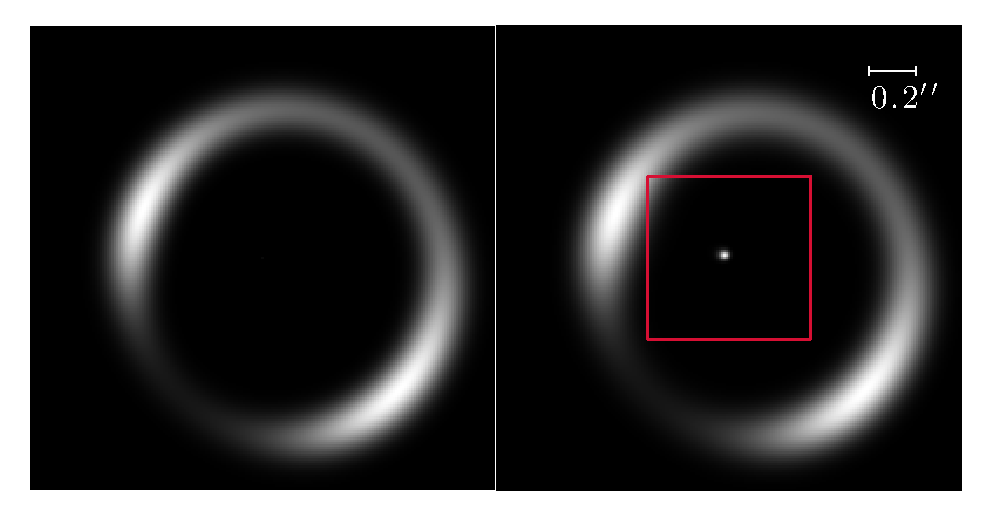
\includegraphics[trim= 0 0 0 0, width=0.45\textwidth]{figures/f_02.eps}
\centering
\end{center}
\caption{ illustration of the central image in 2 cases: 
\label{f:f2}}
\end{figure}


\begin{figure}
\begin{center}
\centering
\includegraphics[trim= 0 0 5 6, clip, width=0.45\textwidth]{figures/f_01.eps}
\centering
\end{center}
\caption{ Model density profiles. The black dashed line shows the dark matter component, with a slope of 0.1, consistent with a projected NFW at the innermost regions. the grey dashed curves show cored-sersic five fits to stellar light profiles of massive galaxies from Ferrarese 2006. The red solid curve shows our cored-power-law model that we use to approximate this stellar component. The solid black line shows the total matter density (dark plus stellar) of our model. 
\label{f:f2}}
\end{figure}




\begin{figure}
\begin{center}
\centering
\includegraphics[trim= 0 0 0 0, width=0.45\textwidth]{figures/f_03.eps}
\centering
\end{center}
\caption{ Significance of detection of the central image as a function of the stellar core size for a 10-hr long ALMA observation. The colors correspond to different slopes of the stellar component. The solid curves correspond to a case without a SMBH while the dashed line show the result of a simulation which includes a $2\times10^8M_{\odot}$ SMBH at its center.
\label{f:f2}}
\end{figure}


\begin{figure}
\begin{center}
\centering
\includegraphics[trim= 0 0 0 0, width=0.45\textwidth]{figures/f_04.eps}
\centering
\end{center}
\caption{ Covariance matrix of parameters for a few different scenarios.
\label{f:f2}}
\end{figure}



\section{Conclusion}

\acknowledgements{
}



\end{document}
